\documentclass[aspectratio=169]{beamer}

% Je kan het lettertype iets vergroten door hierboven optie ``14pt'' toe te
% voegen.

%==============================================================================
% Aanloop
%==============================================================================

%---------- Vormgeving --------------------------------------------------------

\usetheme{hogent}

% Kies hieronder een achtergrondkleur
%\usecolortheme{hgwhite} % witte achtergrond, zwarte tekst
\usecolortheme{hgblack} % zwarte achtergrond, witte tekst

%---------- Packages ----------------------------------------------------------

\usepackage[english]{babel}      % Nederlandse taal: splitsingen, enz.

\usepackage{booktabs}          % Mooie tabellen
\usepackage{multirow,multicol} % Tabelcellen samenvoegen
\usepackage{eurosym}           % Euro symbool

%\usepackage{animate} % GIFS
\usepackage{media9}
\usepackage{fontspec}
\usepackage{multimedia} % Use multimedia instead of media9
\usepackage{hyperref}


%---------- Commando-definities -----------------------------------------------

%---------- Info over de presentatie ------------------------------------------

\title[AI Judge]{AI judge assistant for recognition of jump rope skills in videos.}
\author{Mike De Decker}
\author[MDD]{Mike {De Decker} (\href{mailto:mikeddecker@hotmail.com}
    {mikeddecker@hotmail.com})}
\date{\today}

%==============================================================================
% Inhoud presentatie
%==============================================================================

\begin{document}

%---------- Titelpagina, inhoudstafel -----------------------------------------

{
\setbeamertemplate{background}[imgletter]
    {dd3-boxes-dark.jpg}{H}

\begin{frame}
    \maketitle
\end{frame}
}

%---------- Corpus ------------------------------------------------------------

\begin{frame}
  \frametitle{Diciplines}

  \hspace{0.1cm}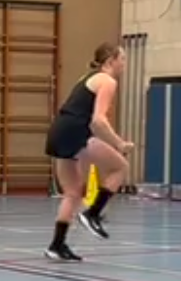
\includegraphics[height=2cm]{speed}
  \hspace{0.1cm}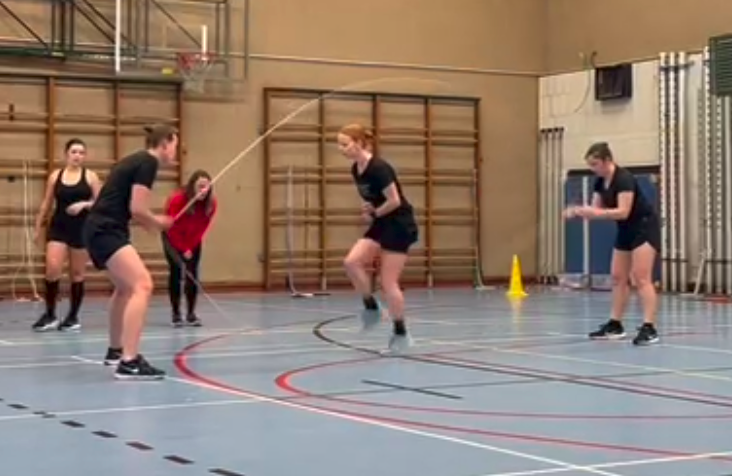
\includegraphics[height=2cm]{ddspeed}
  \hspace{0.1cm}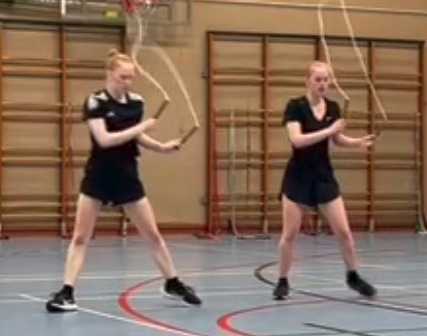
\includegraphics[height=2cm]{sr}
  \hspace{0.1cm}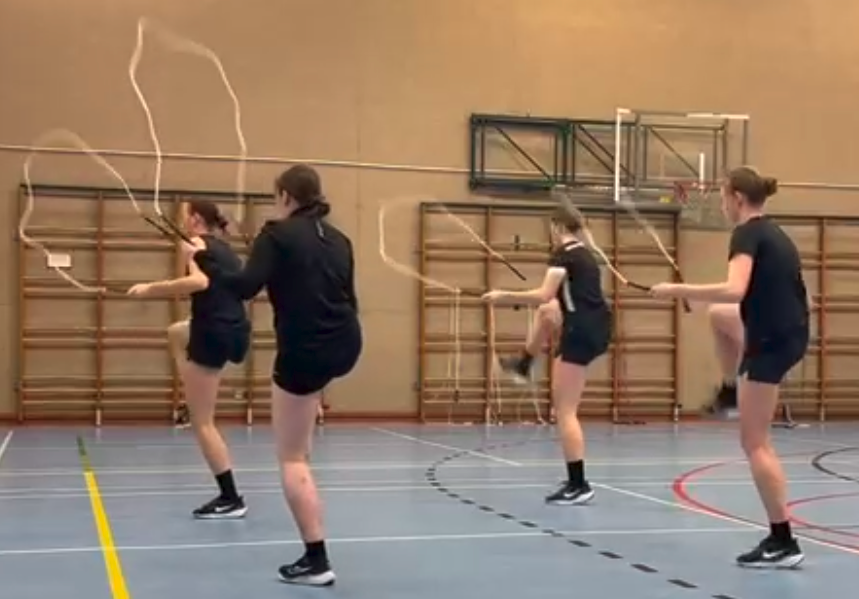
\includegraphics[height=2cm]{sr-team} \\
  \vspace{0.1cm}
  \hspace{0.1cm}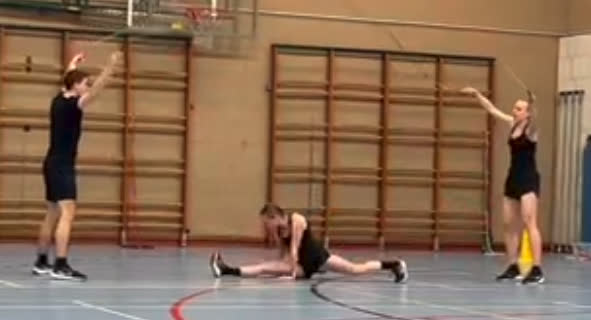
\includegraphics[height=2cm]{dd3}
  \hspace{0.1cm}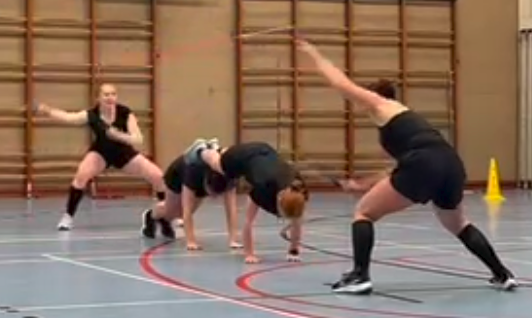
\includegraphics[height=2cm]{dd4}
  \hspace{0.1cm}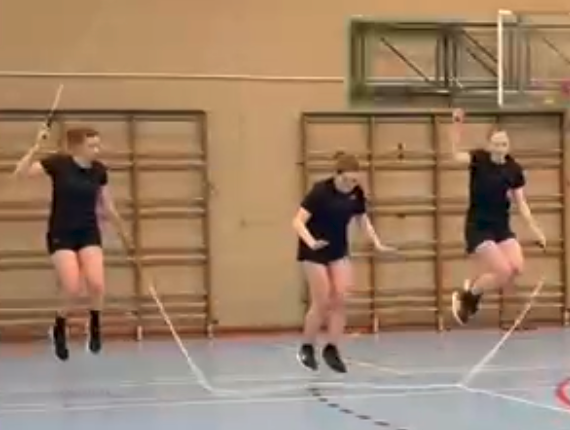
\includegraphics[height=2cm]{cw}

\end{frame}

% \begin{frame}
%   \frametitle{Comparing routines}

%   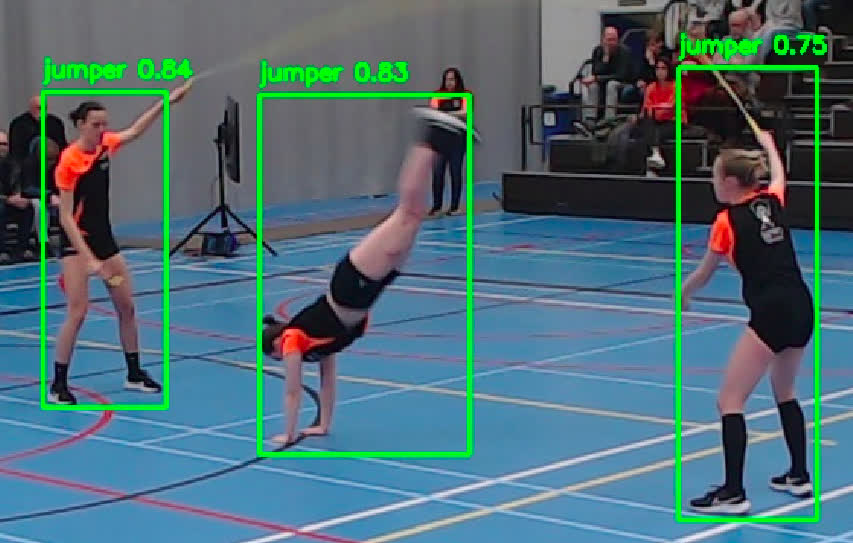
\includegraphics[height=4cm]{dd3-boxes.jpg}
%   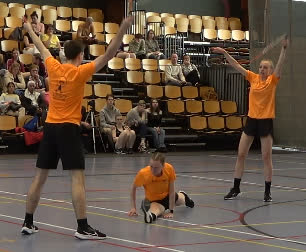
\includegraphics[height=4cm]{dd3-split.jpg}

% \end{frame}

\begin{frame}
  \frametitle{Judges}
  \vspace{-1.5cm}
  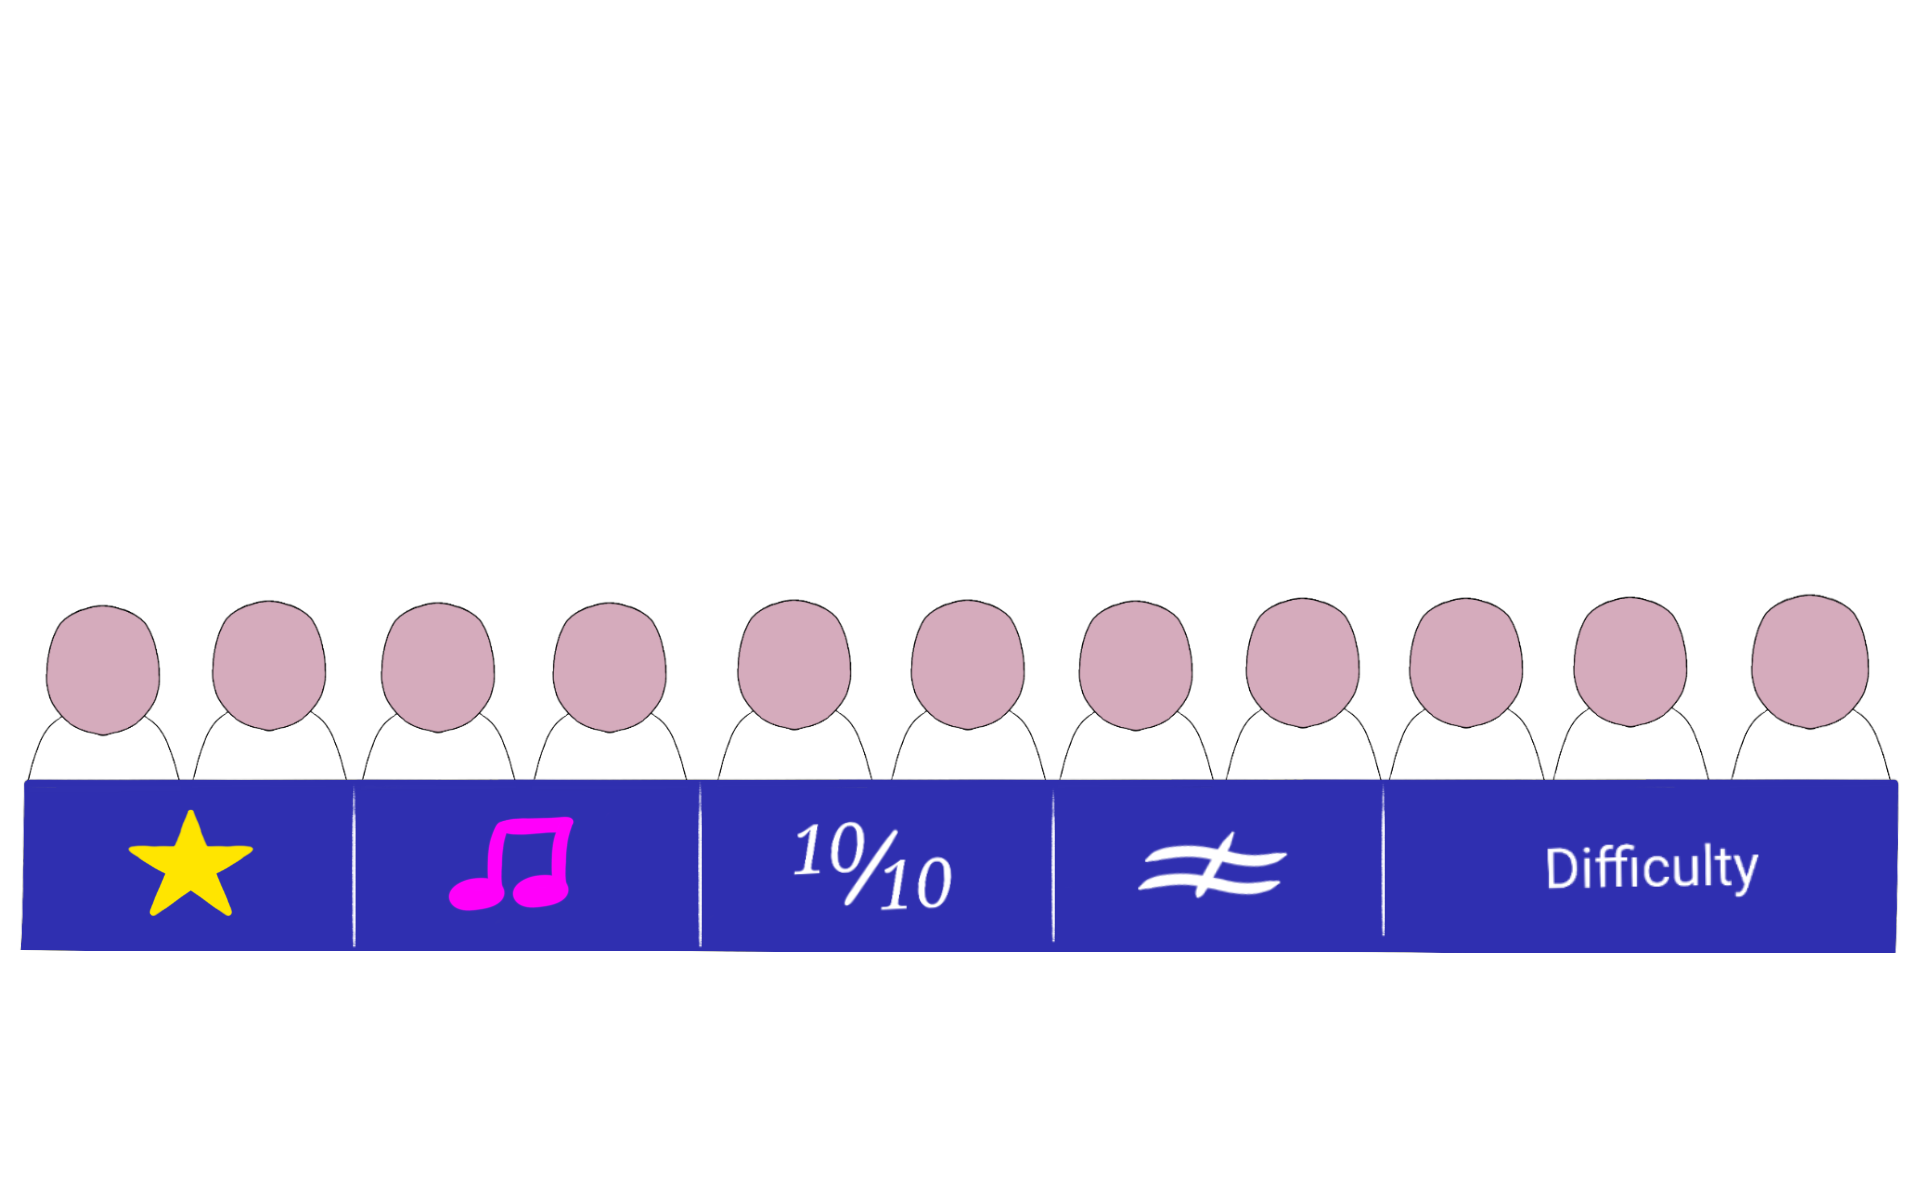
\includegraphics[width=0.9\linewidth]{judges}
  
  % TODO : add cine diffusion link if kept
\end{frame}

\begin{frame}
  \frametitle{Scoring difficulty.}
  \vspace{-0.3cm}
  Using levels [1 -> 8]
  \vspace{0.2cm}

  \begin{columns}[c]
  
    \column{.55\textwidth}
    \hspace{0.2cm} 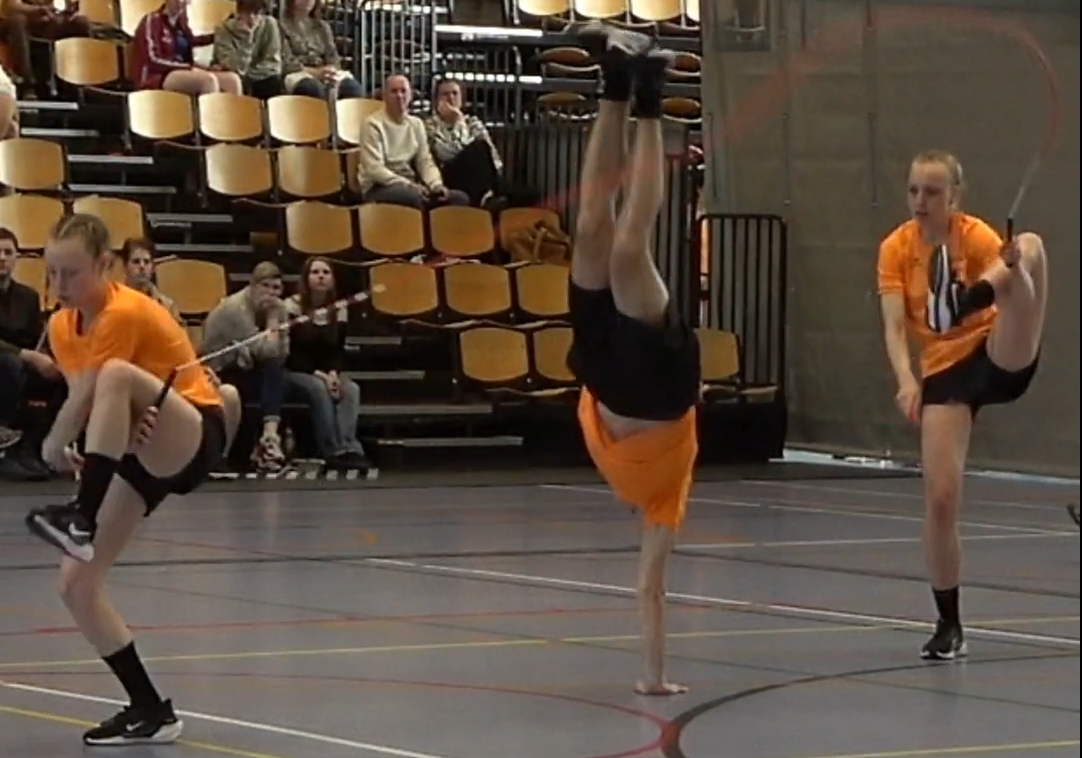
\includegraphics[width=0.85\linewidth]{dd3-1h-hfrog-toad-bw-crouger}

    \column{.45\textwidth}
    Base skill level \\
    + \\
    Turner restrictions \\
    + \\
    Nr of rotations \\
    + \\
    Modifiers (one hand, body rotations...)

  \end{columns}
\end{frame}

\begin{frame}
  \frametitle{AI Judge assistant}

  \begin{columns}[c]
  
    \column{.75\textwidth}
    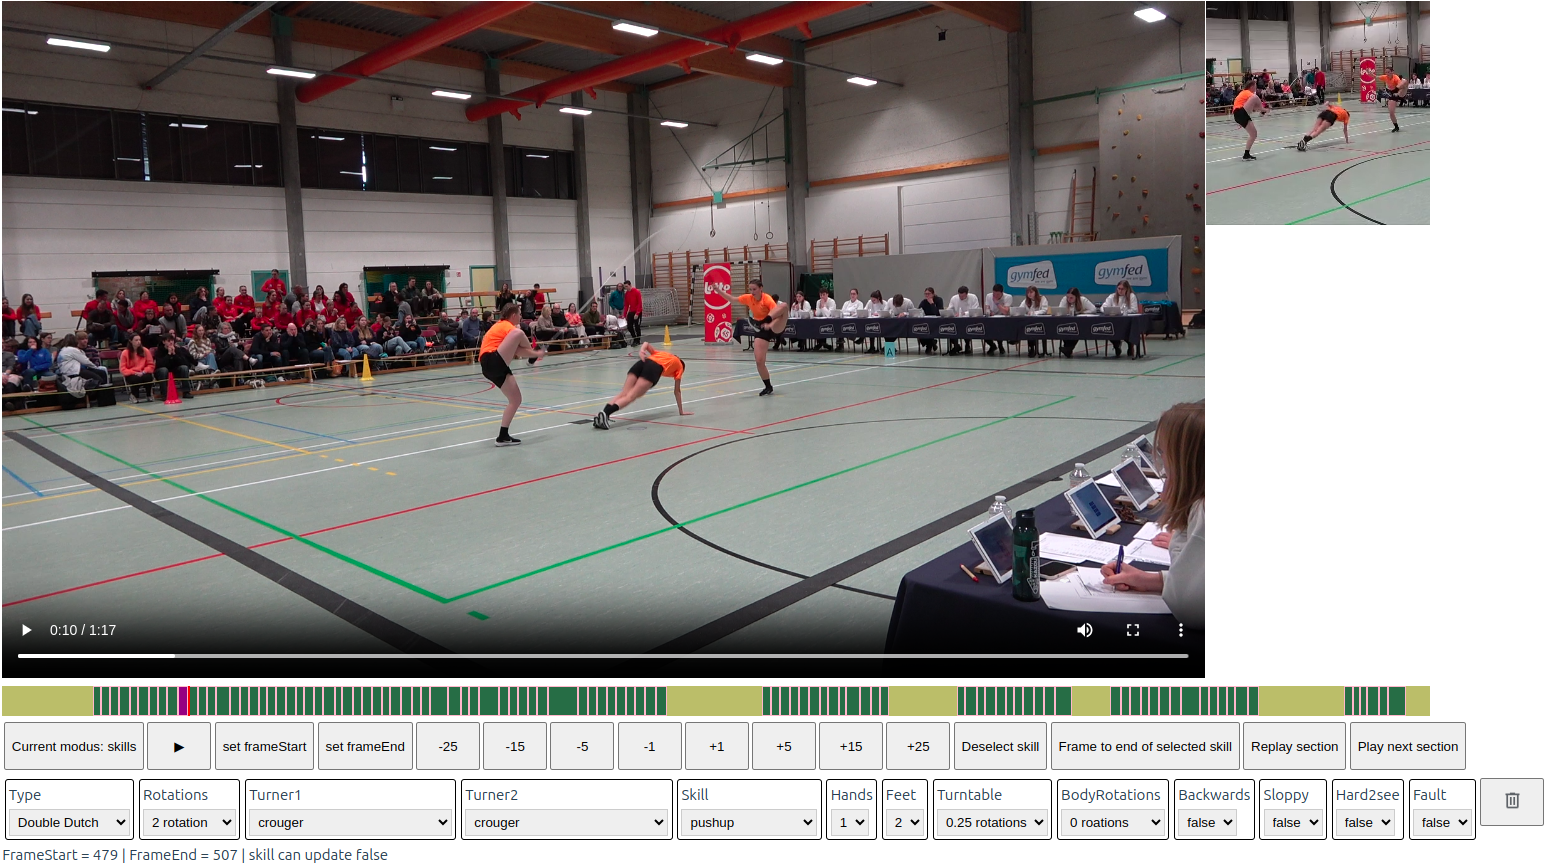
\includegraphics[width=1.0\linewidth]{label-video}

    \column{.25\textwidth}
    \vspace{-1.0cm}
    \begin{enumerate}
      \item localize
      \item segment
      \item recognition
    \end{enumerate}

  \end{columns}
\end{frame}

\begin{frame}
  \frametitle{Jumper localization}

  \begin{columns}[c]
  
    \column{.25\textwidth}
    \vspace{-1.0cm}
    \begin{enumerate}
      \item Full team
      \item Individual
      \item YOLO
    \end{enumerate}

    \column{.75\textwidth}
    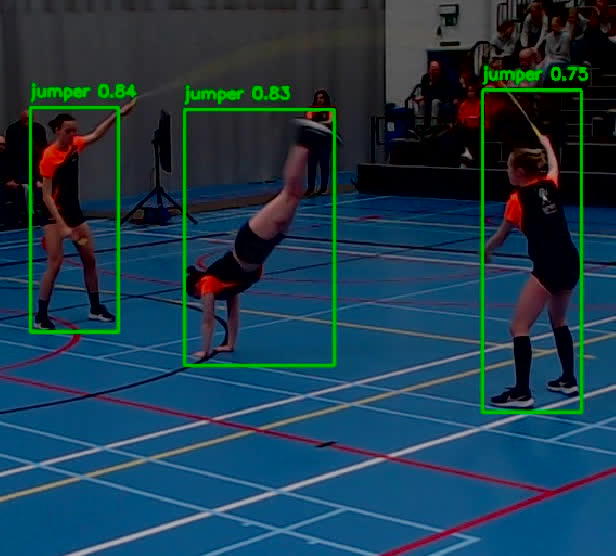
\includegraphics[width=0.6\linewidth]{dd3-boxes-dark.jpg}


  \end{columns}
\end{frame}

\begin{frame}
  \frametitle{Action segmentation}

  \begin{columns}[c]
    
    \column{.3\textwidth}
    \vspace{-1.0cm}
    \begin{enumerate}
      \item 0 or 1
      \item every N frames
      \item Peaks
      \item Transform to an equal length
    \end{enumerate}
    \vspace{1.0cm}
    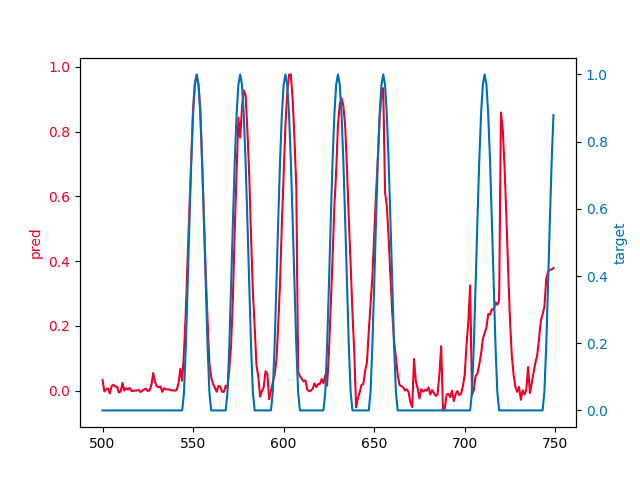
\includegraphics[width=0.7\linewidth]{ai-judge-segment-plot}
    
    \column{.70\textwidth}
    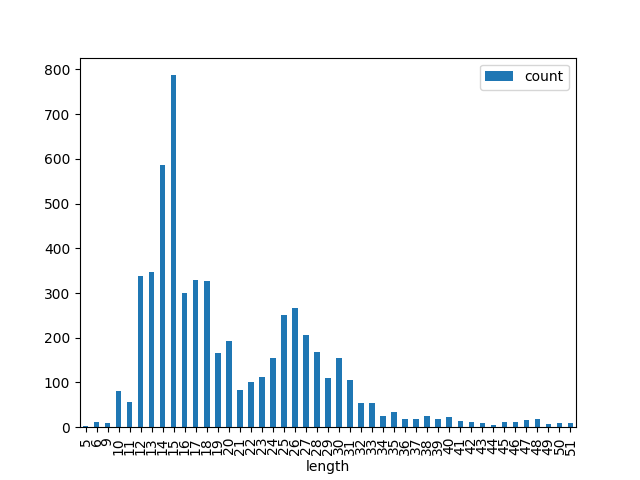
\includegraphics[width=0.8\linewidth]{skilllengths}

  \end{columns}
\end{frame}

\begin{frame}
  \frametitle{Skill recognition}

  \begin{itemize}
    \item Data labels, nr of videos
    \item Up-sampling
    \item 5 classes \& down sampling
    \item Mutiscale Video Transformer
    \item Data augmentation (Mirror)
    \item ResNet (R3D, R2plus1, MC3), SA\_Conv3D\_LSTM, SwinTransformer
  \end{itemize}
\end{frame}


\begin{frame}
  \frametitle{Skill recognition}

  \begin{table}[h!]
    \begin{tabular}{|l|r|r|r|r|}
                \hline       & precision & recall  & f1-score &  support \\ \hline
                     SPAGAAT  &     0.00 &    0.00  &    0.00  &     0.0 \\
                      UNKOWN  &     0.00 &    0.00  &    0.00  &     3.0 \\
                buddy-bounce  &     0.00 &    0.00  &    0.00  &     1.0 \\
                        crab  &     0.68 &    0.89  &    0.77  &    19.0 \\
                        flip  &     0.47 &    0.70  &    0.56  &    10.0 \\
              flip-to-pushup  &     0.00 &    0.00  &    0.00  &     0.0 \\
             footwork-cancan  &     0.00 &    0.00  &    0.00  &     0.0 \\
              footwork-cross  &     0.00 &    0.00  &    0.00  &     0.0 \\
               footwork-kick  &     0.00 &    0.00  &    0.00  &     0.0 \\
               footwork-knee  &     0.00 &    0.00  &    0.00  &     0.0 \\
               footwork-open  &     0.00 &    0.00  &    0.00  &     2.0 \\
                        frog  &     0.98 &    1.00  &    0.99  &    88.0 \\
                  handspring  &     0.67 &    0.40  &    0.50  &     5.0 \\
            \hline
    \end{tabular}
    \caption[Skill class report after weighted losses 1]{Skill class report after weighted losses 1}
    \label{tbl:mvit-class-reports-skills-after-weighted-losses-1}
  \end{table}
\end{frame}

\begin{frame}
  \frametitle{Skill recognition}

  \begin{table}[h!]
    \begin{tabular}{|l|r|r|r|r|}
                \hline       & precision & recall  & f1-score &  support \\ \hline
                        jump  &     0.98 &    0.96  &    0.97  &   444.0 \\
                         kip  &     1.00 &    0.62  &    0.77  &     8.0 \\
                      kopkip  &     0.00 &    0.00  &    0.00  &     2.0 \\
                      pushup  &     0.92 &    0.99  &    0.95  &   100.0 \\
                         rad  &     0.00 &    0.00  &    0.00  &     4.0 \\
           return from power  &     0.85 &    0.90  &    0.87  &   108.0 \\
                     rol2kip  &     0.44 &    1.00  &    0.61  &     7.0 \\
                        roll  &     0.00 &    0.00  &    0.00  &     2.0 \\
                      rondat  &     0.50 &    0.43  &    0.46  &     7.0 \\
                       split  &     0.89 &    0.50  &    0.64  &    16.0 \\
                        stut  &     0.00 &    0.00  &    0.00  &     4.0 \\
                     suicide  &     0.69 &    0.90  &    0.78  &    10.0 \\
                       swift  &     0.00 &    0.00  &    0.00  &     0.0 \\
            \hline
    \end{tabular}
    \caption[Skill class report after weighted losses 2]{Skill class report after weighted losses}
    \label{tbl:mvit-class-reports-skills-after-weighted-losses}
  \end{table}

\end{frame}

\begin{frame}
  \frametitle{F1 accuracies}
  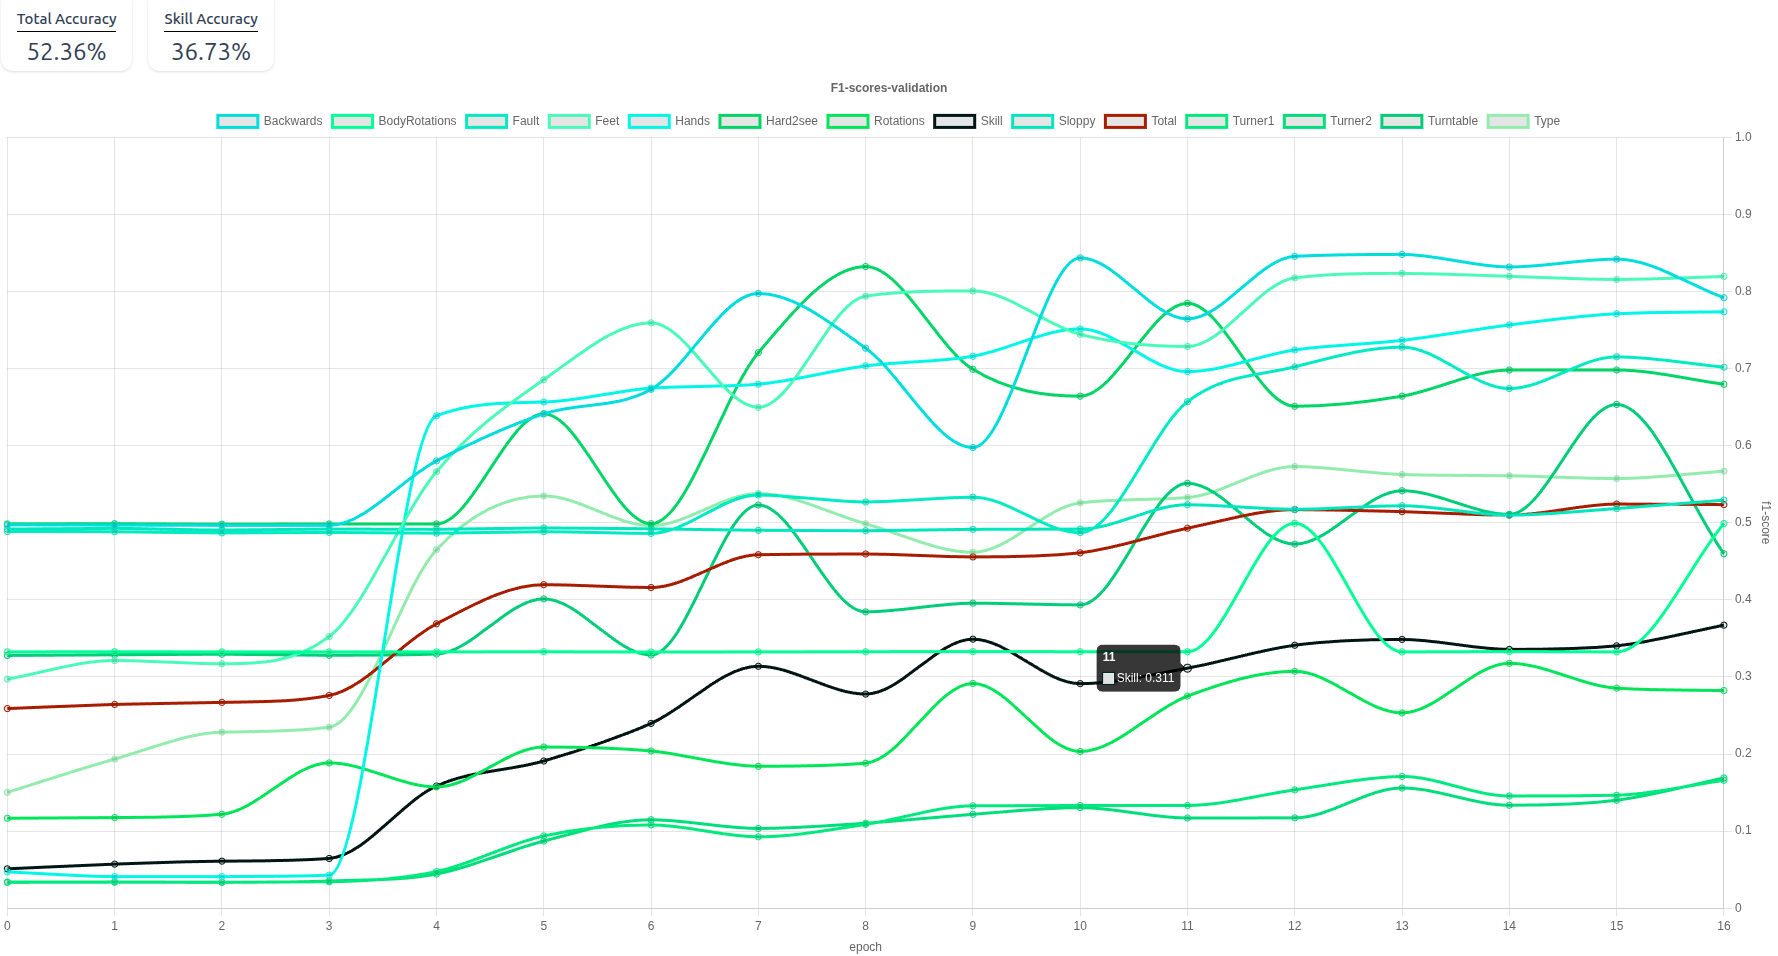
\includegraphics[width=0.9\linewidth]{f1-accuracies}
\end{frame}

\begin{frame}
  \frametitle{Compare models}
  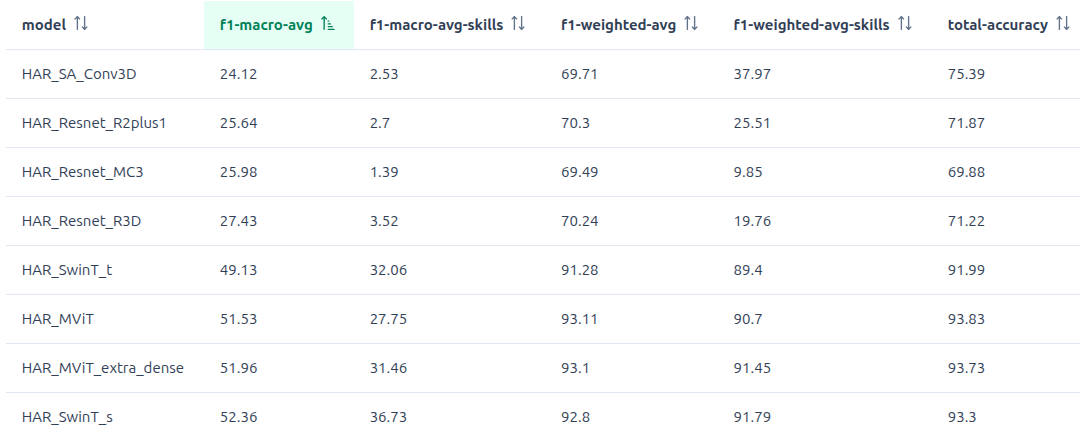
\includegraphics[width=0.9\linewidth]{modelcomparison}
\end{frame}

\begin{frame}
  \frametitle{Comparing judge scores}

  -20.94\% MViT extra dense  \\
  -21.68\% MViT  \\
  -23.83\% SwinT s  \\
  -27.72\% SwinT t  \\
  -38.85\% Resnet MC3  \\
  -53.09\% Resnet R3D  \\
  +47.15\% Resnet R2plus1  \\
\end{frame}


\begin{frame}
  \frametitle{AI Judge assistant}

  \begin{columns}[c]
    \column{.33\textwidth}
    \centering{Localize}
    \column{.33\textwidth}
    \centering{Segment}
    \column{.33\textwidth}
    \centering{Recognize}
  \end{columns}

  \begin{columns}[c]
  
    \column{.33\textwidth}
    \begin{center}
      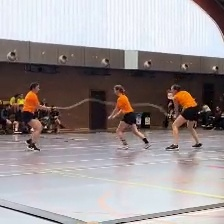
\includegraphics[width=0.8\linewidth]{ai-judge-localize-crop}
    \end{center}
    
    \column{.33\textwidth}
    \begin{center}
      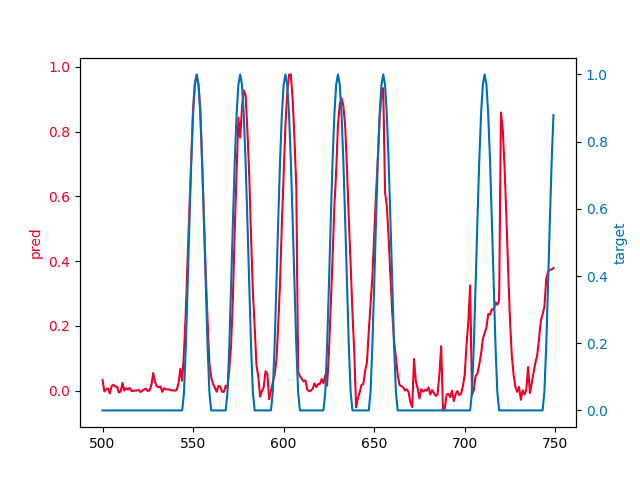
\includegraphics[width=1.0\linewidth]{ai-judge-segment-plot}
    \end{center}
    % \vspace{0.kcm}
    \begin{center}
      
\includegraphics[width=0.8\linewidth]{ai-judge-segments}
    \end{center}

    \column{.33\textwidth}
    
    \begin{center}
        cartwheel \\
        handstand \\
        2 rotations \\
        1 hand \\
        2 feet \\
        ... 
    \end{center}
      
  \end{columns}


\end{frame}

\begin{frame}{Video example}
  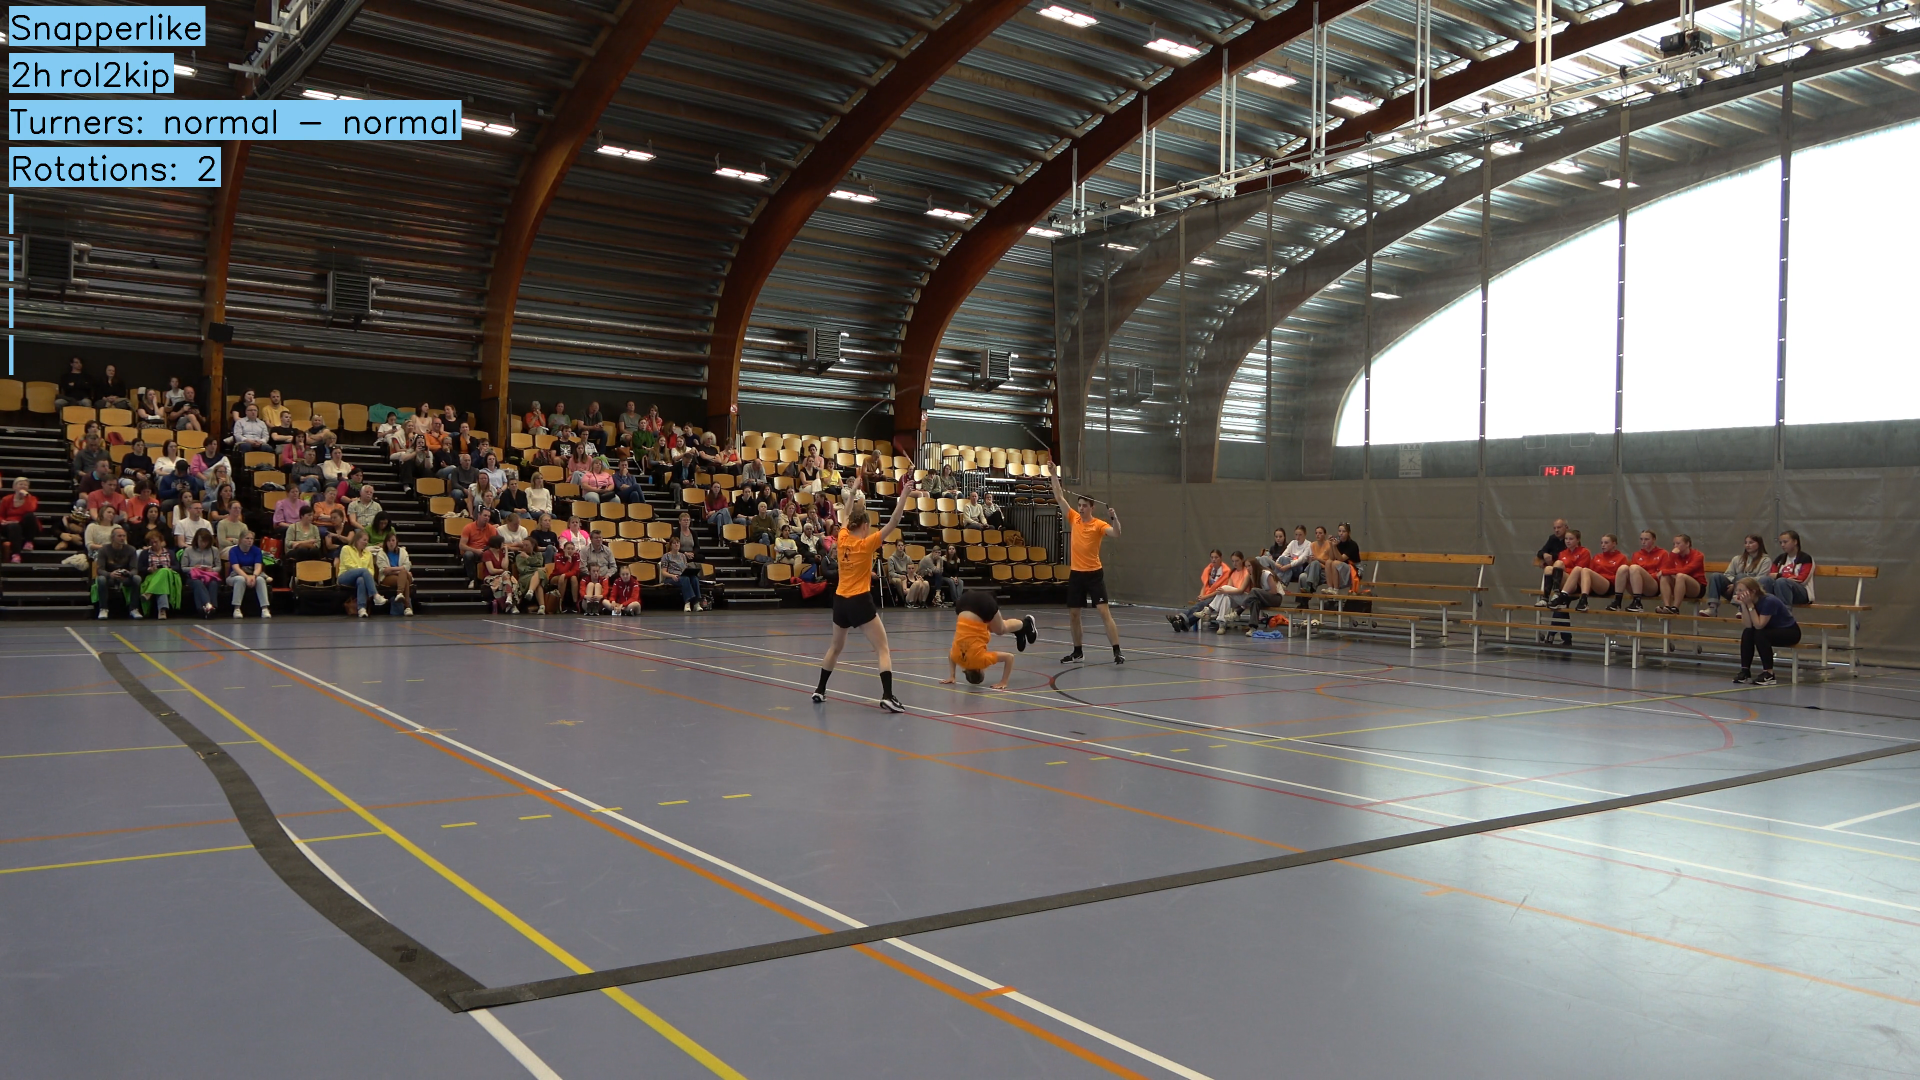
\includegraphics[width=0.6\linewidth]{dd3-predicted-skill} 
  
  \hypertarget{autoplay}{} % A dummy target
  \href{run:dd3-annotated.mp4}{\beamergotobutton{Click to play the video}}
\end{frame}


\end{document}
